% !TEX root = MutationTestingSurvey.tex

\section{Mutation Testing Process}
\label{sec:process}

	\begin{figure}
	\centering
		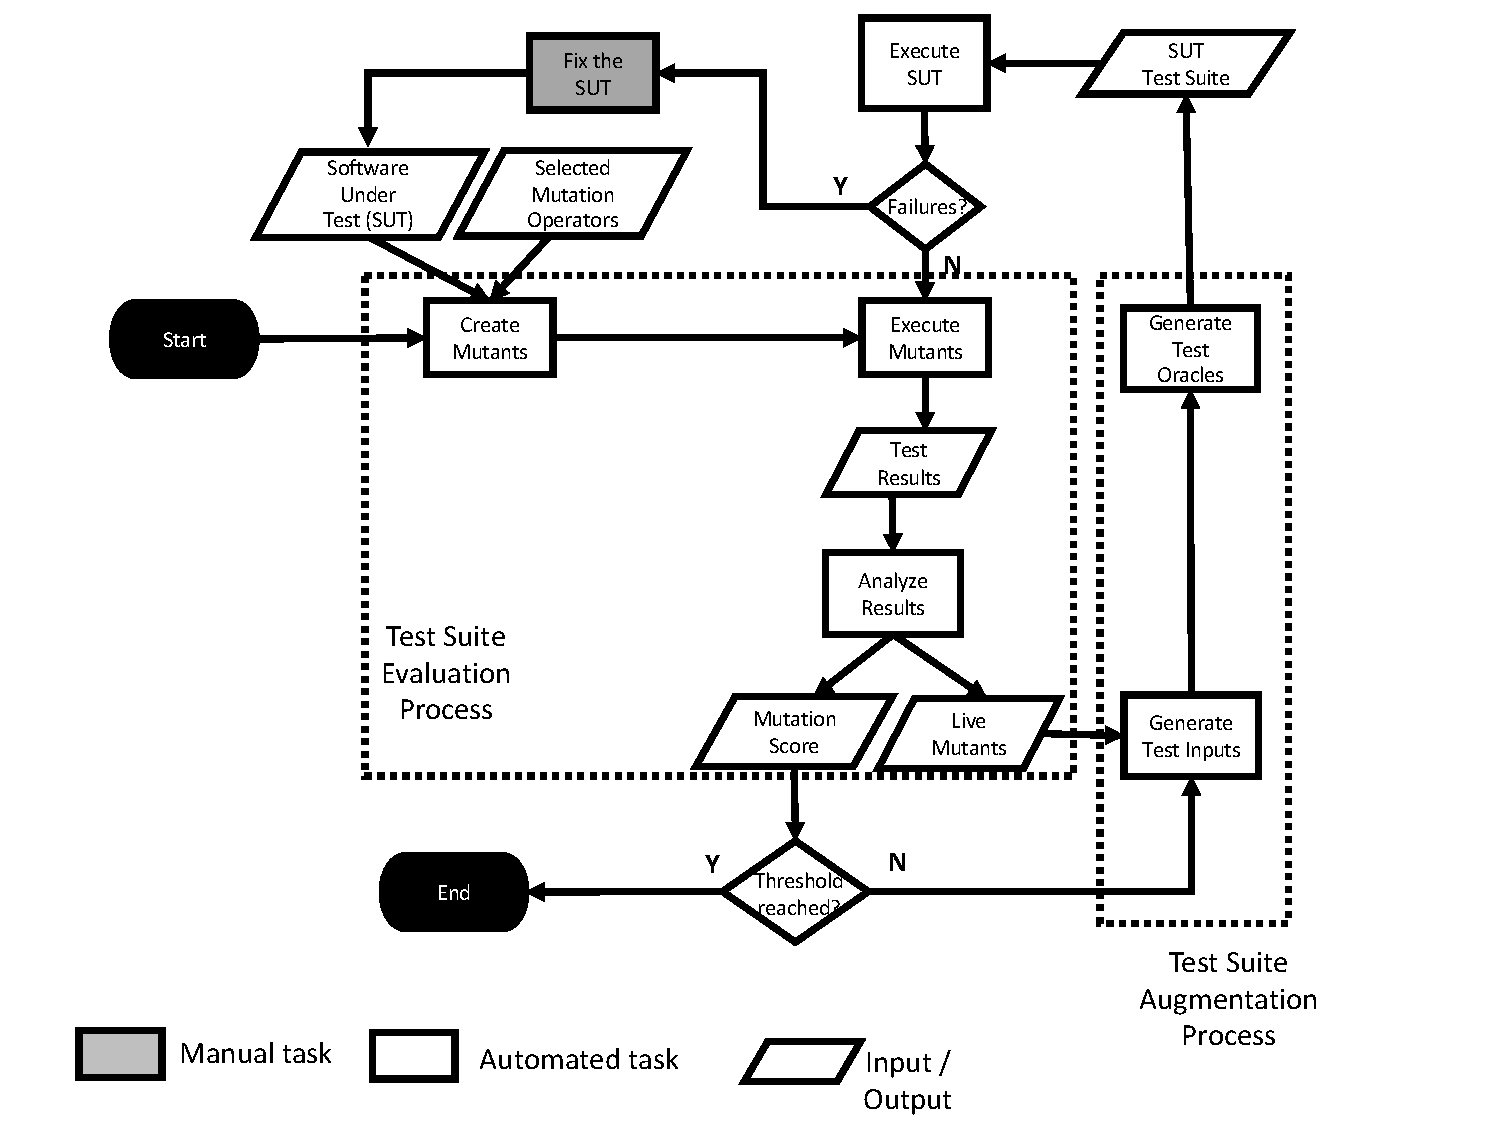
\includegraphics[width=\textwidth]{images/process}
		\caption{Mutation Testing Process.}
		\label{fig:code:process}
	\end{figure}

Figure \ref{fig:code:process} shows the reference code-driven mutation testing process that will be considered in this book. The process depicted in Figure \ref{fig:code:process} has been inspired by the mutation testing process described in related work \cite{offutt2001mutation,papadakis2019mutation}. The process is based on two main sub-processes, \emph{test suite evaluation} and \emph{test suite augmentation}, which are described in Sections~\ref{sub:test_suite_evaluation}~and~\ref{sub:test_suite_augmentation}, respectively.


\subsection{Test Suite Evaluation} % (fold)
\label{sub:test_suite_evaluation}

The Test Suite Evaluation process concerns the automatic generation of modified versions (i.e., the mutants) of the software under test (SUT) and the evaluation of the quality of the SUT test suite. It consists of three activities: \emph{create mutants}, \emph{execute mutants}, and \emph{analyze results}. 
These activities are typically automated by toolsets that often include strategies to address scalability issues. 

Figure~\ref{fig:code:process} provides an overview of the test suite evaluation process.
It starts with engineers providing the SUT and a set of mutation operators selected to be considered for creating modified versions of the software. 
The set of available mutation operators depends on the toolset implementing the test suite evaluation process. 
A set of mutation operators implemented by most of the existing toolsets consists of the relational (ROR), logical (LCR), arithmetic (AOR), absolute (ABS) and unary insertion (UOI) operators \cite{rothermel1996experimental}. 
%Several research paper target the definition of mutation operators; relevant for this ESA activity are works on the definition of mutants for floating point operators \cite{dan2012semantic}, operators synthesized by processing the revision history of C projects \cite{brown2017care}, mutation operators targeting memory operations \cite{wu2017memory}, deletion operators \cite{delamaro2014designing}, operators targeting components integration \cite{grechanik2016mutation}. Finally, recent attention has been put towards the development of higher-order mutation operators \cite{harman2010manifesto,ghiduk2017higher}. First order mutation seeds faults generated by a single syntactic change to the original program. Higher order mutation combines first order mutants to simulate more complex faults, motivated by a desire to capture subtle faults \cite{jia2009higher}. 
Section~\ref{sec:operators} provides an overview of the mutation operators defined in the literature that can be applied in the context of space and embedded systems.

In the test suite evaluation process, the activity \emph{create mutants} concerns the application of the mutation operators to the source code of the SUT; it leads to the generation of modified versions of the SUT (i.e., the mutants) that should be compiled and then executed against the test suite to evaluate the test suite quality. 
The \emph{execution of mutants} implies the execution of the test suite of the SUT against all the generated mutants. 
%Optimizations for the execution of mutants concern the scalability of the execution process and 
%the identification at run-time of equivalent and redundant mutants.

Unfortunately, the activity \emph{create mutants} leads to a high number of mutants to be generated, which, in turn, leads to scalability issues due to the compilation and execution of the different program versions generated. Recent surveys provide an overview of existing optimization techniques~\cite{ferrari2018systematic};
the most relevant optimization approaches target the reduction of the number of mutants to be compiled and executed, 
the reduction of the compilation iterations, the reduction of the execution time, and the identification of equivalent and redundant mutants.

To reduce the number of program versions that need to be compiled and executed, existing approaches automatically select subsets of the generated mutants. Two main mutant selection approaches have been defined: the selection of representative mutation operators and the random selection of mutants \cite{zhang2010operator}. The first approach consists of the empirical identification of a subset of mutation operators that is sufficient to predict the mutation score \cite{siami2008sufficient,barbosa2001toward}. The second approach consists of randomly selecting a certain percentage of mutants from the generated ones \cite{wong1995reducing}, possibly with a uniform distribution of the different mutation operators \cite{zhang2010operator}. Empirical results with academic case studies \cite{zhang2010operator} show that the first approach is not superior to random selection when selecting the same number of mutants. Other work \cite{zhang2013operator} show that the combination of operator-based selection and random sampling leads to better results since it leads to high mutation score (above 98\%) while reducing the average mutation testing time to 6.54\%. The use of higher-order mutants is another solution to reduce the overall number of mutants. 
Other optimizations are framework specific, for example, Mull limits mutations to reachable code \cite{hariri2018srciror}. Section~\ref{sec:opt:selection} provides an overview of mutant selection approaches.

To reduce the time spent in the compilation of the generated mutants, mutant schemata \cite{untch1993mutation} consist of encoding all the mutants in a single file and parametrize the mutant execution so that mutants are compiled in a single pass and selected at runtime. Section~\ref{sub:compileTime} provides an overview of compile-time optimization approaches.

Another optimization that speeds up the compilation of mutants concerns the identification of equivalent and redundant mutants. Equivalent mutants are mutants that behave as the original program, while redundant mutants are mutants that lead to the same test failures. 
To detect if a program and one of its mutants are
equivalent is undecidable~\cite{Budd:1982}; however, heuristics to partially address the problems have been defined in the literature.
Trivial compiler optimization might be adopted to detect both equivalent and redundant mutants; it relies on the idea that source code that leads to the same program behaviour often belongs to the same optimized compiled code \cite{papadakis2015trivial}. Other approaches concern the adoption of symbolic execution \cite{papadakis2012mutation,kurtz2015static} and the runtime monitoring of the SUT (e.g., mutants that lead to the same execution paths are likely equivalent \cite{schuler2013covering}). Finally, Shin et al. proposed the \emph{distinguishing mutation adequacy criterion}, which aims to ensure that the test suite includes enough different test inputs so that every mutant is distinguished by each other, if feasible~\cite{shin2017theoretical}. 
Solutions to address the problem of identifying equivalent and redundant mutants are detailed in Sections~\ref{sec:opt:equivalent} and~\ref{sec:opt:redundant}, respectively.






A well-known optimization to \emph{reduce execution time} is the split-stream optimization, which consists of generating a modified version of the SUT that creates multiple processes (one for each mutant) only when the mutated code is reached \cite{tokumoto2016muvm}. With split-stream, the code shared among multiple mutants is executed only once thus saving time and resources. Other execution optimizations consist of minimizing the number of processes being created by sharing one single process among mutants that bring the system into the same state \cite{wang2017faster}.
Section~\ref{sec:opt:execution} provides an overview of techniques to reduce execution time and, more generally, address run-time scalability issues.



The \emph{analysis of test results} concerns the identification of mutants that lead to the failure of at least one test case of the SUT test suite; these mutants are said to be \emph{killed}. Mutants that do not lead to the failure of any test case are said to be \emph{live mutants}. The identification of killed and live mutants enable the definition of a mutation adequacy criterion as follow, \emph{a test suite is mutation-adequate if all mutants are killed by at least one test of the test suite}. 
Also, the percentage of killed mutants is used to quantitatively measure the quality of a test suite. This measure is referred to as \emph{mutation score}.
Because of equivalent and redundant mutants, mutation-adequacy is difficult to achieve while the mutation score might not be representative of test suites quality~\cite{papadakis2016threats}. Section~\ref{sub:mutationscore} provides an overview of solutions addressing the problems related to the computation of the mutation score.



The capability of a test case to kill a mutant often depends on the observability of the system state. 
To overcome the limitations due to observability, different strategies for distinguishing program executions (i.e, to determine if the execution of two test cases led to different results) have been defined. These strategies are known as strong, weak, firm, and flexible mutation coverage.
\emph{Strong mutation coverage} indicates that the computation of the mutation score is based on the percentage of mutants identified by test failures, i.e., based on difference between the expected and the observed output of the system.  
\emph{Weak mutation coverage} consists of verifying if the state of the system has been altered, with respect to the original code, after the execution of the mutated statement. 
\emph{Firm mutation coverage} consists of verifying if the change in the state of the system propagates after the mutated code, e.g., at function boundaries. 
\emph{Flexible mutation coverage} consists of checking if the mutated code leads to object corruption \cite{mateo2012validating}. The main difference between these four coverage strategies is that only strong mutation coverage enables engineers to assess the quality of test cases in their entirety, i.e., by evaluating both the capability of triggering an erroneous behavior and the capability of reporting the erroneous behaviour thanks to complete test oracles. The other strategies only evaluate the capability of the test suites of triggering the erroneous behavior. 

% subsection test_suite_evaluation (end)

\subsection{Test Suite Augmentation} % (fold)
\label{sub:test_suite_augmentation}

The test suite augmentation process concerns the definition of test cases that kill live mutants.
It consists of four activities \emph{Identify Test Inputs}, \emph{Generate Test Oracles}, \emph{Execute the SUT}, \emph{Fix the SUT}. The first two activities concern the definition of new test cases.
The third activity, i.e., the execution of the SUT, enables engineers to determine if the newly defined test cases spot faults not identified by the original test suite. 
Finally, the repair of the SUT (i.e., activity \emph{Fix the SUT}) is performed in the case of test failures.
In this book we focus on the techniques that can be applied to automate the first two activities (i.e., \emph{Identify Test Inputs}, and \emph{Generate Test Oracles}).
 
The identification of test inputs has the objective of identifying inputs for the SUT that make the SUT produce an output that is different than the one produced by one of the mutants not killed by the existing test suite.
%To this end, mutants could be ranked according to their importance in order to ensure that, for a given test budget, the most relevant mutants are considered first. MuRanker \cite{namin2015muranker}, for example, ranks mutants according to their predicted difficulty and complexity in being detected. 
Existing work investigated the adoption of the KLEE symbolic execution engine \cite{holling2016nequivack} and the use of bounded model checking \cite{riener2011test}. Other work combines dynamic symbolic execution (DSE) with search-based software testing (SBST) to generate test inputs that lead to strong mutations \cite{harman2011strong}. 

The generation of test oracles, instead, should lead to the generation of executable code instructions (e.g., assertions) that verify if the output generated by the SUT is correct.
In the case of automated test generation approaches, a state-of-the-art approach consists of the generation of assertions that verify the value of variables that enable the killing of mutants \cite{fraser2011mutation}. 
In the case of test suite generation for mutation testing, the generation of test oracles could be driven by the comparison of the outputs generate by the SUT and by the specific mutants targeted during test generation~\cite{Staats2012}.

In all the cases, the generated oracles need to be validated, more precisely we need to ensure that the values expected by the oracles do not reflect a failure triggered by the test case (e.g, an erroneous value being returned). Such validation activity is typically performed manually by the engineers because it should be based on domain knowledge and system specifications. Indeed specifications are generally written in natural language because, to reduce development costs, only few components of the system are specified using formal languages.
Approaches that support engineers in the analysis of generated oracles exists and might be considered to speed up the process~\cite{PastoreICSE2015}.

Test failures observed after updating the test suites should be investigated by the engineers who are expected to fix the SUT.
If test failures are not observed, engineers evaluate the quality of the newly generated test suite by executing it against the mutants and by observing the mutation score achieved. 

Section~\ref{sec:testGeneration} provides an overview of approaches for the automated generation of test cases.

% subsection test_suite_augmentation (end)
